%*******************************************************************************
%****************************** Second Chapter *********************************
%*******************************************************************************

\chapter{L'étanchéité à l'air}

\ifpdf
    \graphicspath{{Chapter2/Figs/Raster/}{Chapter2/Figs/PDF/}{Chapter2/Figs/}}
\else
    \graphicspath{{Chapter2/Figs/Vector/}{Chapter2/Figs/}}
\fi


\section{Différentes normes}

%NIT 255 chap 3
L'expression de l'étanchéité à l'air peut se faire de plusieurs façons. Pour les réglementations PEB nous parlerons de perméabilité à l'air sous une différence de pression de 50 Pa. Cette mesure est exprimée en débit de fuite par unité de surface, elle est notée $\stackrel{.}{v}_{50}$ et est exprimée en $[m^3/(h\cdot m^2)]$.
La norme NBN EN 13829 nous décrit un taux de renouvellement d'air qui est noté $n_{50}$ et sera exprimé en $h{-1}$

\begin{figure}[ht]
\centering
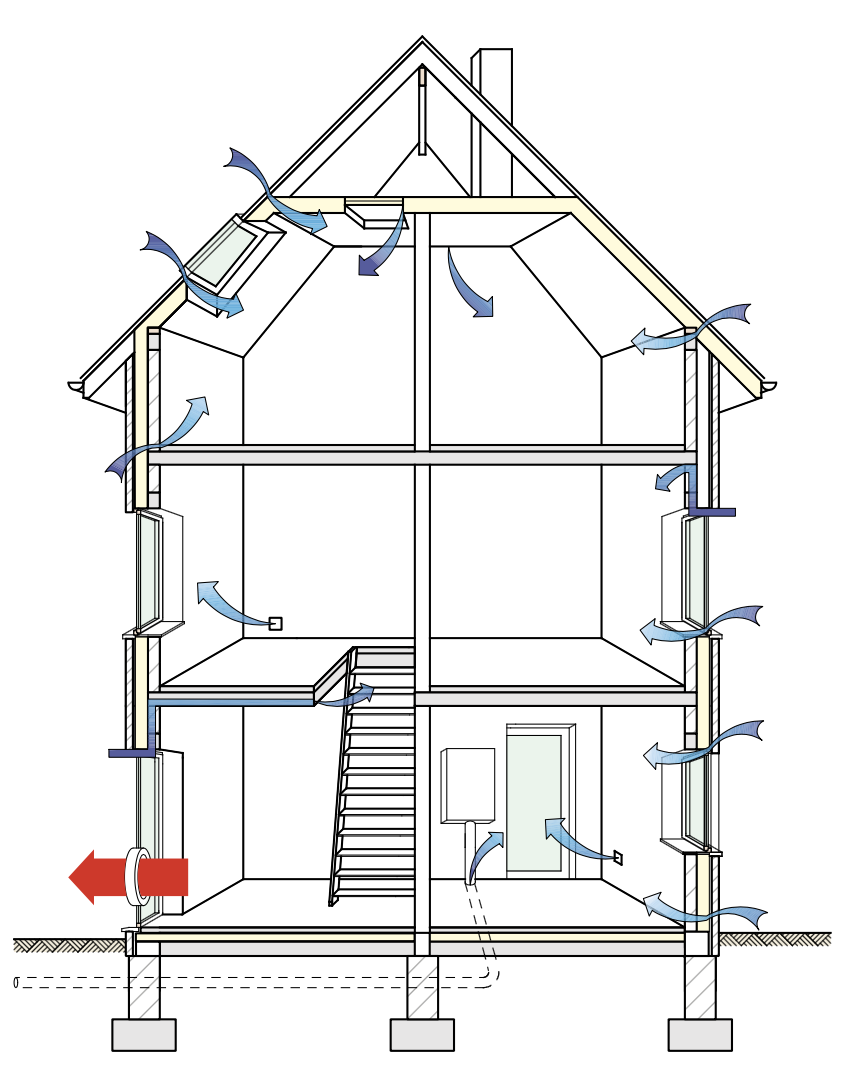
\includegraphics[width=0.5\textwidth]{Airpaths}
\caption{\label{Airpath} Exemples des endroits par ou l'air peut s'infiltrer (NIT 255 p20)}
\end{figure}


\subsection{Perméabilité à l'air}
La perméabilité à l'air dépend d'un débit de fuite ($\stackrel{.}{V}_{50}$ au travers de l'enveloppe du bâtiment testée sous une différence de pression de 50 Pa. La perméabilité dépend aussi de la surface totale de l'enveloppe du bâtiment ($A_{test}$), sans prendre en compte les murs mitoyens avec des espaces chauffés. Ceci est illustré à la figure \ref{SurfaceEnveloppe}.

$$\stackrel{.}{v}_{50}= \dfrac{\stackrel{.}{V}_{50}}{A_{test}}$$

\begin{figure}[ht]
\centering
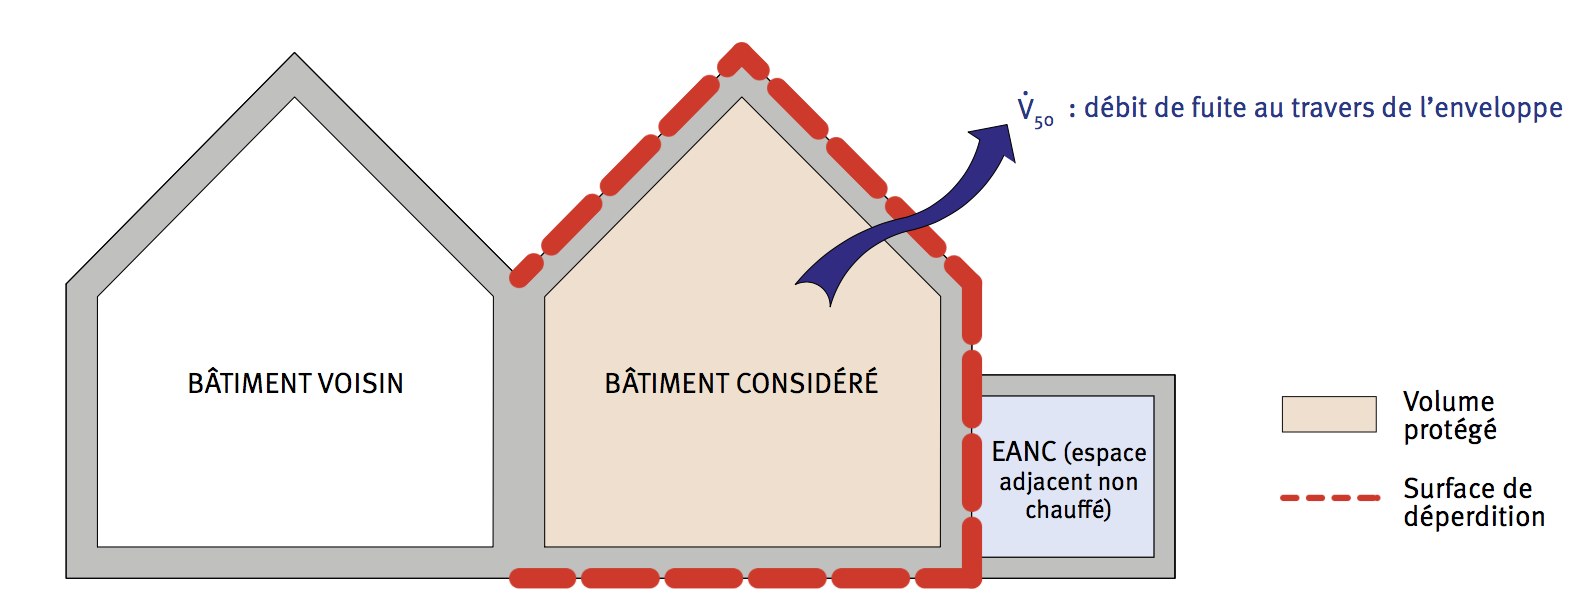
\includegraphics[width=1.0\textwidth]{SurfaceEnveloppe}
\caption{\label{SurfaceEnveloppe} Visualisation de la surface d'enveloppe d'un bâtiment (NIT 255 p20)}
\end{figure}

\subsection{Taux de renouvellement d'air}
Le taux de renouvellement d'air dépend aussi du débit de fuite ($\stackrel{.}{V}_{50}$) mais contrairement à la perméabilité d'air elle ne dépendra pas de la surface d'enveloppe mais du volume intérieur du bâtiment ($V_{int}$). Ceci est illustré à la figure \ref{VolumeInterieur}

$$n_{50} =  \dfrac{\stackrel{.}{V}_{50}}{V_{int}}$$

\begin{figure}[ht]
\centering
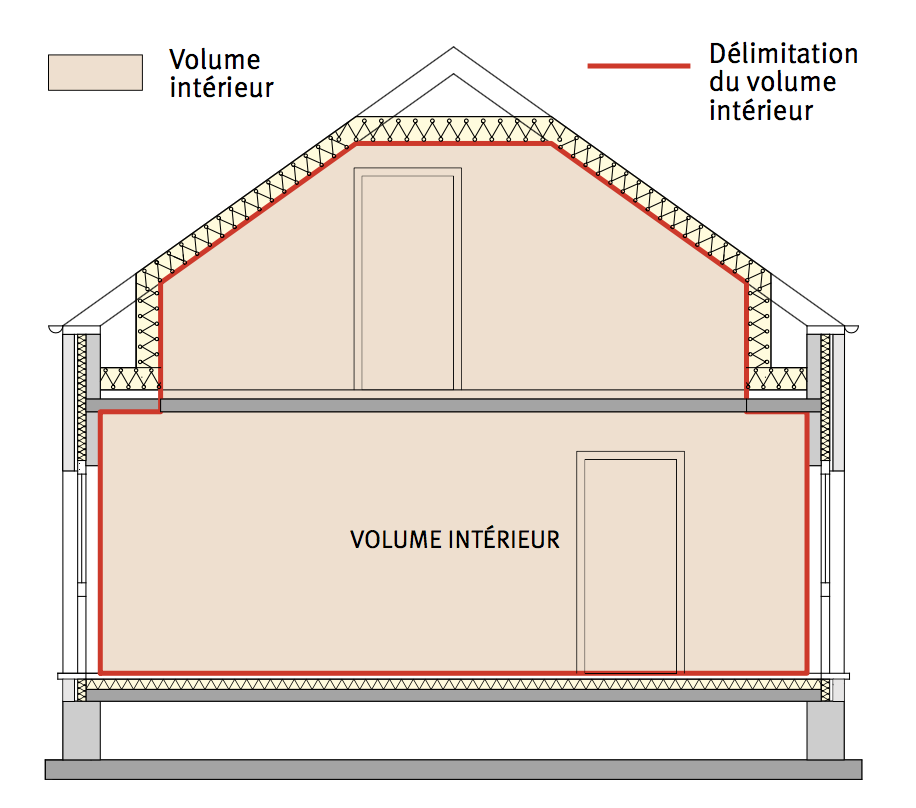
\includegraphics[width=0.5\textwidth]{VolumeInterieur}
\caption{\label{VolumeInterieur} Visualisation du volume intérieur d'un bâtiment (NIT 255 p21)}
\end{figure}

\subsection{Comparaison de la réglementation PEB et le label 'Passif'}

\begin{figure}[ht]
\centering
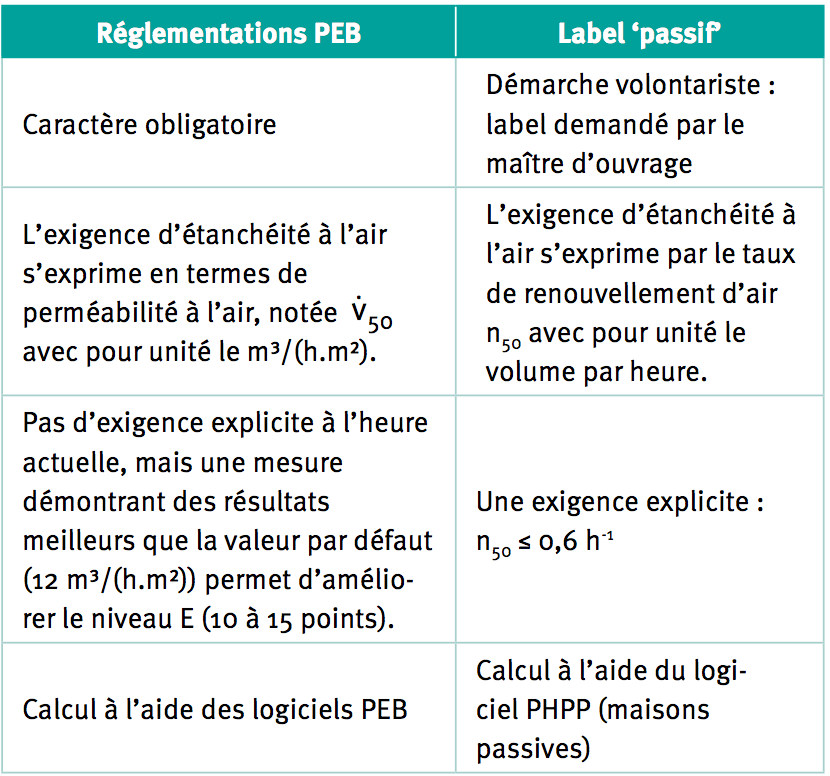
\includegraphics[width=0.5\textwidth]{TableauComparatif}
\caption{\label{TableauComparatif} Comparaison (NIT 255 p23)}
\end{figure}


\section{Comment se déroule un test d'infiltrométrie}
\begin{figure}[ht]
\centering
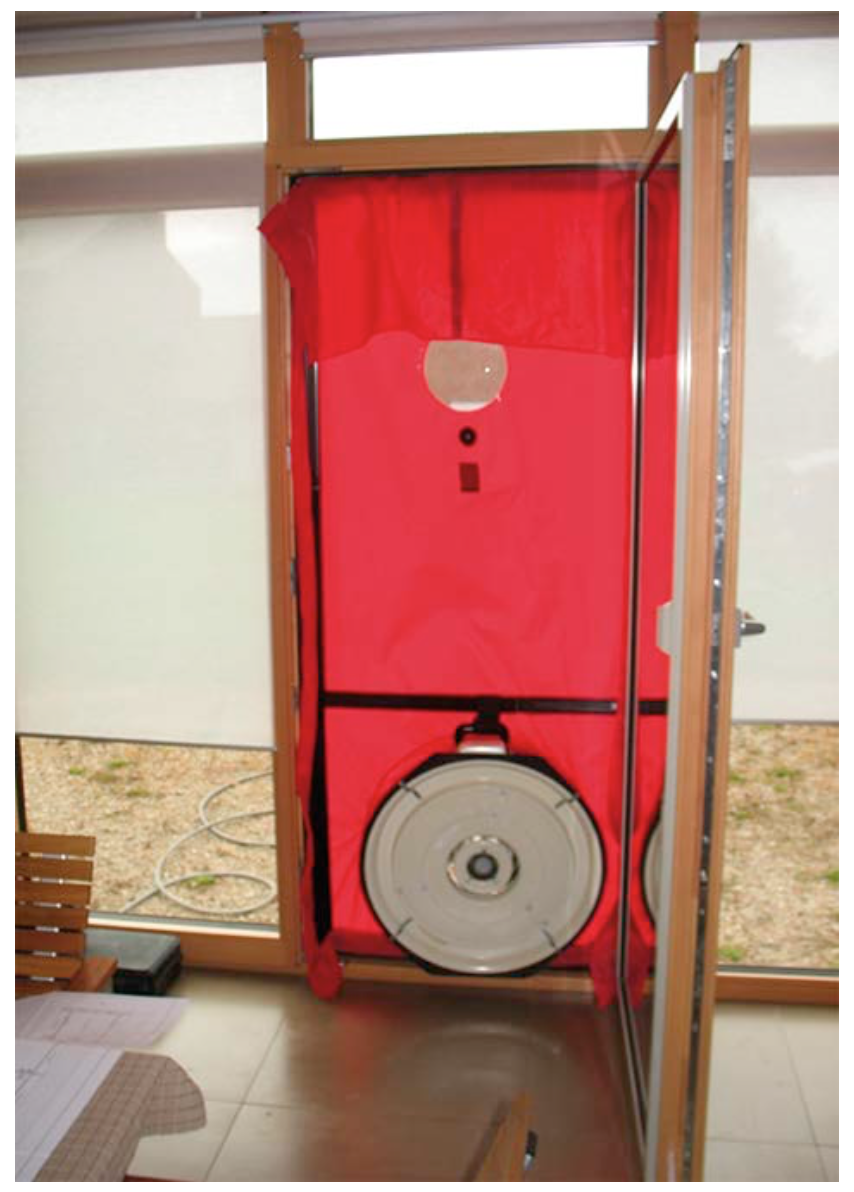
\includegraphics[width=0.5\textwidth]{Blowerdoor}
\caption{\label{Blowerdoor} Porte de pressuration (NIT 255 p101)}
\end{figure}


